%; whizzy paragraph -pdf xpdf -latex ./whizzypdfptex.sh
%; whizzy-paragraph "^\\\\begin{frame}"
% latex beamer presentation.
% platex, latex-beamer でコンパイルすることを想定。 

%     Tokyo Debian Meeting resources
%     Copyright (C) 2009 Junichi Uekawa
%     Copyright (C) 2009 Nobuhiro Iwamatsu

%     This program is free software; you can redistribute it and/or modify
%     it under the terms of the GNU General Public License as published by
%     the Free Software Foundation; either version 2 of the License, or
%     (at your option) any later version.

%     This program is distributed in the hope that it will be useful,
%     but WITHOUT ANY WARRANTY; without even the implied warreanty of
%     MERCHANTABILITY or FITNESS FOR A PARTICULAR PURPOSE.  See the
%     GNU General Public License for more details.

%     You should have received a copy of the GNU General Public License
%     along with this program; if not, write to the Free Software
%     Foundation, Inc., 51 Franklin St, Fifth Floor, Boston, MA  02110-1301 USA

\documentclass[cjk,dvipdfmx,12pt]{beamer}
\usetheme{Tokyo}
\usepackage{monthlypresentation}

\setbeamertemplate{footline}{\hskip1mm\insertshortdate\hfill\hbox{\insertpagenumber /\insertdocumentendpage }\hspace*{1mm}\vskip1mm}

%  preview (shell-command (concat "evince " (replace-regexp-in-string "tex$" "pdf"(buffer-file-name)) "&")) 
%  presentation (shell-command (concat "xpdf -fullscreen " (replace-regexp-in-string "tex$" "pdf"(buffer-file-name)) "&"))
%  presentation (shell-command (concat "evince " (replace-regexp-in-string "tex$" "pdf"(buffer-file-name)) "&"))

%http://www.naney.org/diki/dk/hyperref.html
%日本語EUC系環境の時
\AtBeginDvi{\special{pdf:tounicode EUC-UCS2}}
%シフトJIS系環境の時
%\AtBeginDvi{\special{pdf:tounicode 90ms-RKSJ-UCS2}}

\newenvironment{commandlinesmall}%
{\VerbatimEnvironment
  \begin{Sbox}\begin{minipage}{1.0\hsize}\begin{fontsize}{8}{8} \begin{BVerbatim}}%
{\end{BVerbatim}\end{fontsize}\end{minipage}\end{Sbox}
  \setlength{\fboxsep}{8pt}
% start on a new paragraph

\vspace{6pt}% skip before
\fcolorbox{dancerdarkblue}{dancerlightblue}{\TheSbox}

\vspace{6pt}% skip after
}
%end of commandlinesmall


\title{OSC 2013 Tokyo/Fall \\東京エリアDebian勉強会}
\subtitle{第105回 2013年10月度}
\author{野島 貴英 nozzy@debian.or.jp}
\date{2013年10月20日}
\logo{
\includegraphics[width=8cm]{image200607/openlogo-light.eps}}

\begin{document}

\frame{\titlepage{}}

%\section{}

\begin{frame}{Agenda}
 \begin{itemize}
  \item Wheezy!
 \item パッケージ数/開発者数推移
  \item Jessie! 
  \item その他
  \item イベントのご紹介
  \item 質疑応答
 \end{itemize}
\end{frame}

\begin{frame}{本資料は?}
\begin{itemize}
\item 東京エリアDebian勉強会ホームページの10月の案内\\
  \url{http://tokyodebian.alioth.debian.org/2013-10.html}\\にて公開してます。
\item プレゼン資料のダウンロードリンクです:\\
   \url{http://tokyodebian.alioth.debian.org/pdf/debianmeetingresume201310-presentation.pdf}
\end{itemize}
\end{frame}

\begin{frame}{自己紹介}
\begin{itemize}
\item 野島 貴英 (Takahide Nojima)
\item Twitter: @nozzy123nozzy
\item 東京エリアDebian勉強会
\item 主に東京エリアDebian勉強会に出没、たまに開催のお手伝い/発表もしてます
\end{itemize}
\end{frame}

\begin{frame}
\begin{center}
\LARGE{Debian topic update}
\end{center}
\end{frame}

\begin{frame}{どこからのupdate?}
\begin{center}
\Large{前回の2013年2月OSC Tokyo/Springからのアップデートとなります。}
\end{center}
\end{frame}


\begin{frame}

\begin{center}
\LARGE
Wheezy!
\end{center}

\end{frame}


\begin{frame}{Wheezyリリース!!}

\begin{center}
\LARGE
2013/5/4 Debian 7.0(Whezzy)リリース
\end{center}
\url{http://www.debian.org/News/2013/20130504}
\end{frame}


\begin{frame}{Wheezy入手の国内 mirror}

日本国内で入手するには、

\begin{itemize}
\item インストール用イメージについては↓\\
  \begin{itemize}
  \item {i386/amd64 Debian GNU/Linux用イメージ} \\
    \url{http://cdimage.debian.or.jp/}
  \item {Debian GNU/kFreeBSD用イメージ} \\
    \url{http://cdimage.debian.or.jp/kfreebsd.html}
  \end{itemize}
\item パッケージ群のftpミラーサイト\\
  \url{http://ftp.jp.debian.org/debian/}
\end{itemize}  
\end{frame}

\begin{frame}{Wheezyインストール方法}

Wheezyのインストールについては、\\
Debian wheezy -- インストールガイド\\
\url{http://www.debian.org/releases/stable/installmanual}\\
をご覧くださいませ。
\end{frame}

\begin{frame}{Wheezyリリースノートについて}
ところで、
\begin{itemize}
\item Wheezyの変更点やら、
\item Squeeze $\rightarrow$ Wheezyへのアップグレードのやり方と注意点
\end{itemize}
については、\\
「Debian 7.0 -- リリースノート」\\
\url{http://www.debian.org/releases/stable/releasenotes}\\
を見てねーっ
\end{frame}

\begin{frame}{さらにWheezyアップデートの状況}

\begin{itemize}
\item 2013/6/15にてWheezyの1stアップデート(Debian 7.1)\\
\url{http://www.debian.org/News/2013/20130615}\\
33個のセキュリティ修正と、60個のパッケージを更新。\\
(kernel側は数々のバグfix及びdrmは3.4.47対応、deboostrapの次期リリースのjessie対応追加、その他パッケージはバグフィックスが主)
\item 2013/10/12にてWheezyの2ndアップデート(Debian 7.2)\\
\url{http://www.debian.org/News/2013/20131012}
58個のセキュリティ修正と、102個のパッケージを更新、6個のパッケージを廃止\\
(kernel側は3.2.51対応及びdrmは3.4.61対応、iceweasel17未対応のパッケージを排除、その他パッケージはバグフィックスが主)
\end{itemize}

\end{frame}

\begin{frame}
\begin{center}
\LARGE
パッケージ数/開発者数推移
\end{center}
\end{frame}

\begin{frame}{パッケージ数}
\begin{itemize}

\item Wheezy(stable)\\
バイナリパッケージ数: 35985 {\color{red}+7862}\\
ソースパッケージ数  : 17172 {\color{red}+2567}\\
\item Jessie(testing)\\ 
バイナリパッケージ数: 38308 {\color{red}+2141}\\
ソースパッケージ数  : 18998 {\color{red}+1666}\\
\item Sid(unstable)\\ 
バイナリパッケージ数: 40373 {\color{red}+1865}\\
ソースパッケージ数  : 20236 {\color{red}+1465}\\
\end{itemize}
(増減数は前回OSCの時のstable/testing/unstableからの差分)
\end{frame}

% Wheezyパッケージ数は:
% \small{\url{http://ftp.debian.org/debian/dists/wheezy/main/binary-amd64/Packages.gz}にてzegrep '^Package: 'して数える。}}
% Wheezyソースパッケージ数は:
% \small{\url{http://ftp.debian.org/debian/dists/wheezy/main/source/Sources.gz}にてzegrep '^Package: 'して数えた。}}
% Jessieパッケージ数は:
% \small{\url{http://ftp.debian.org/debian/dists/jessie/main/binary-amd64/Packages.gz}にてzegrep '^Package: 'して数えた。}}
% Jessieソースパッケージ数は:
% \small{\url{http://ftp.debian.org/debian/dists/jessie/main/source/Sources.gz}にてzegrep '^Package: 'して数えた。}}
% sidパッケージ数は:
% \small{\url{http://ftp.debian.org/debian/dists/sid/main/binary-amd64/Packages.gz}にてzegrep '^Package: 'して数えた。}}
% sidソースパッケージ数は:
% \small{\url{http://ftp.debian.org/debian/dists/sid/main/source/Sources.gz}にてzegrep '^Package: 'して数えた。}}


\begin{frame}{開発者数}
\begin{itemize}
\item 2013年02月\\
Debian Developer 約1743名 \\
Debian Maintainer 約185名
\item 2013年10月\\
Debian Developer 約1776名 {\color{red}+33}\\
Debian Maintainer 約183名 {\color{blue}-2}\\

\item 参考2013年7月時点で:61ヶ国{2012年6月と比較して\color{red}+2ケ国}\\
日本人  50名 (アクティブメンバ 35名)

\end{itemize}
\end{frame}
% ddの数は、\url{https://db.debian.org/}でカウント。
% DMの数は、\url{https://nm.debian.org/public/people}から、Debian Maintainerの数
% 国別、アクティブ/非アクティブの情報は\url{http://www.perrier.eu.org/weblog/2013/07/27}のblog記事から

\begin{frame}
\begin{center}
\LARGE
Jessie!
\end{center}
\end{frame}


\begin{frame}{ところでJessie}

 Wheezyも出たことですし、次のDebian のメジャーリリースのコードネームは\\

 \begin{center}
 \LARGE
 Jessieだ
 \end{center} 

\end{frame}

\begin{frame}{Jessie Freeze予定!}

 \begin{center}
 \LARGE
 Freeze予定:2014年11月5日\\
 23:59 UTC
 \end{center}

\end{frame}
% See. https://lists.debian.org/debian-devel-announce/2013/10/msg00004.html

\begin{frame}{Jessie Release Goalその1}

リリースゴールの提案が2013/9/11-9/30までの間募集されました。

将来リリースゴールとするかを検討中の一覧(なお、すでにreleaseチームにより検討から落とされたものは排除済み):\\
\begin{itemize}
\item SysV用の起動スクリプトを持つパッケージは、もれなくsystemdにも対応する。
\item ELFバイナリの堅牢化(Hardening)が不十分と報告されているパッケージをなおす (Wheezyから引き続き)
\item debian/rulesファイルは CC/CXXフラグを外部から指定出来るようにする
(要はCC=foo CXX=bar dpkg-buildpackageが出来るようにメンテする)
\item clangもgccの代わりにコンパイラとして利用できるようにする。
\end{itemize}

\end{frame}
\begin{frame}{Jessie Release Goalその2}

続き:
\begin{itemize}
\item すべてのパッケージをpiupartsにて検証済みにする。
\item クロスコンパイルが容易に出来るように整備する(Multiarchはこの一環)
\item 140個の基本的なコマンドのパッケージは、クロスコンパイラを用意すれば、そのままターゲットのアーキテクチャ用のバイナリパッケージが作れるようにする。
\item ユーザがSELinuxをより簡単に使えるようにする。
\item より完全なUTF-8対応
\end{itemize}

\end{frame}

\begin{frame}{JessieのReleseについての情報源}

 \begin{itemize}
 \item Debian Relase Management\\
  \url{http://release.debian.org/}
 \item  Bits from the Release Team (Jessie freeze info)\\
 \url{https://lists.debian.org/debian-devel-announce/2013/10/msg00004.html}
 \end{itemize}

\end{frame}

% 情報ソースは先と同様。また、詳細の説明は、
% 募集時のページにある
% https://wiki.debian.org/ReleaseGoals

\begin{frame}
\begin{center}
\LARGE{その他のトピック}
\end{center}
\end{frame}

\begin{frame}{DPL選挙 in 2013}
\begin{center}
\LARGE
今年のDPL(Debian Project Leader)は、\\
Lucas Nussbaumさんが当選されました。\\
(ID: lucas)
\end{center}
lucasのプロフィールについては↓\\
\url{http://en.wikipedia.org/wiki/Lucas_Nussbaum}
選挙時の声明↓\\
\url{http://www.debian.org/vote/2013/platforms/lucas}
\end{frame}

\begin{frame}{Debian 20歳}
\begin{center}

\Large{2013年8月16日。Debian 20歳。}\\
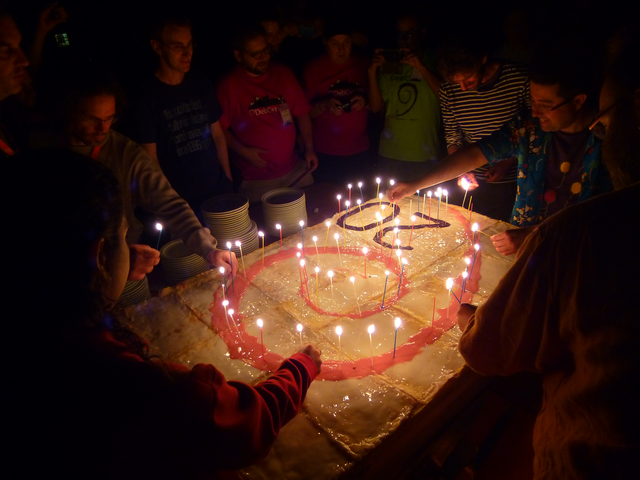
\includegraphics[width=0.8\hsize]{image201310/debian-20years.png}
\end{center}
\end{frame}
% debian-20years.pngの画像は以下からダウンロード
% lucusのプレゼン資料
% http://www.lucas-nussbaum.net/blog/wp-content/uploads/2013/10/owf.pdf

\begin{frame}{最近のDebianのパッケージ開発のトレンド(その1)}
\begin{center}
\Large{グループでパッケージ開発が主流に!}\\
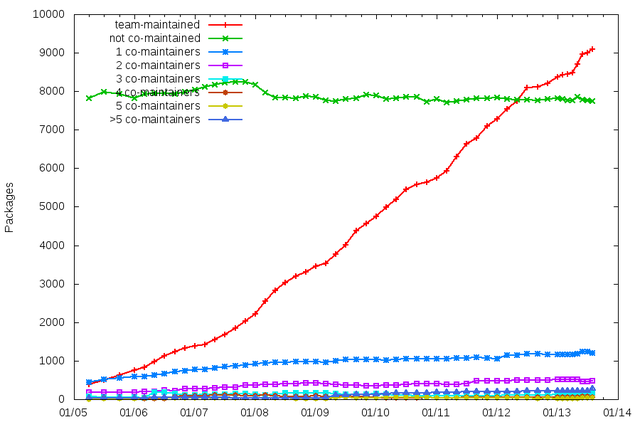
\includegraphics[width=0.8\hsize]{image201310/debian-dev-group.png}
\end{center}
\end{frame}
% debian-dev-group.pngの画像は以下からダウンロード
% lucusのプレゼン資料
% http://www.lucas-nussbaum.net/blog/wp-content/uploads/2013/10/owf.pdf

\begin{frame}{最近のDebianのパッケージ開発のトレンド(その2)}
\begin{center}
\Large{VCSはgitが主流}\\
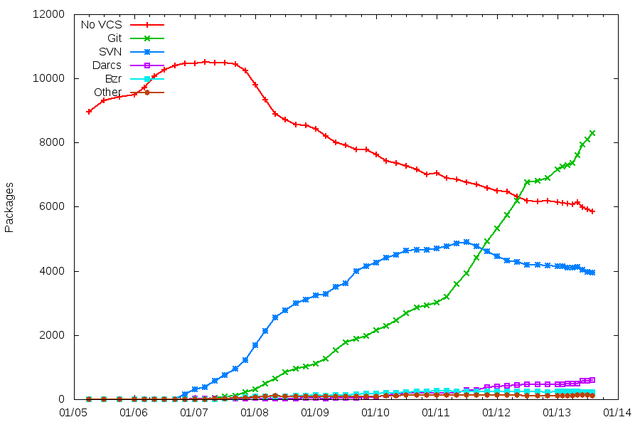
\includegraphics[width=0.8\hsize]{image201310/debian-dev-git-major.png}
\end{center}
\end{frame}
% debian-dev-git-major.pngの画像は以下からダウンロード
% lucusのプレゼン資料
% http://www.lucas-nussbaum.net/blog/wp-content/uploads/2013/10/owf.pdf

\begin{frame}{最近のDebianのパッケージ開発のトレンド(その3)}
\begin{center}
\Large{dhによるパッケージ開発が主流}\\
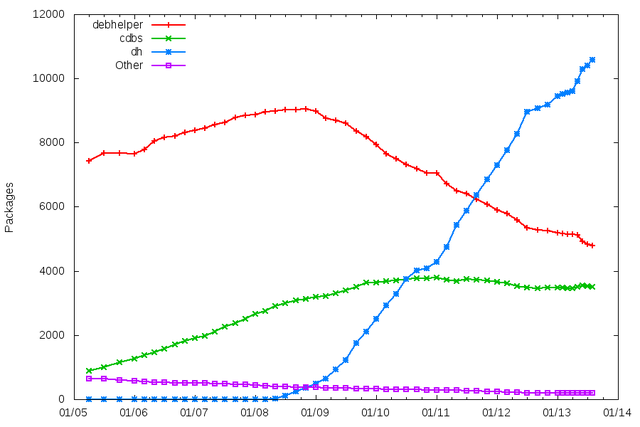
\includegraphics[width=0.8\hsize]{image201310/debian-dev-dh.png}
\end{center}
\end{frame}
% debian-dev-git-major.pngの画像は以下からダウンロード
% lucusのプレゼン資料
% http://www.lucas-nussbaum.net/blog/wp-content/uploads/2013/10/owf.pdf

\begin{frame}{Debianパッケージ開発のお供にいくつか}

ソースコードに関して充実してまいりました。
\begin{itemize}
\item ソースコード検索\\
\url{http://codesearch.debian.net}\\
(エンジンのソースは:\url{https://github.com/debiancodesearch/dcs} )\\
\item ソースコード閲覧\\
\url{http://sources.debian.net/}
\item 参考:ソースパッケージに含まれるパッチトラッカ\\
\url{http://patch-tracker.debian.org/}
\end{itemize}
\end{frame}

\begin{frame}
\begin{center}
\LARGE{Debian カンファレンス}
\end{center}
\end{frame}

\begin{frame}{Debian Conference 2013}
 今回はスイスで2013/8/11-8/18まで開催されました。

\begin{center}

\includegraphics[width=0.8\hsize]{image201310/DebConf13-logo.png}
\end{center}

\end{frame}
%DebConf13-logo.pngは、http://debconf13.debconf.org/artwork.xhtmlより。
%CC BY-SA 3.0とのこと。

\begin{frame}{Debian Conference 2013の様子}

  \begin{itemize}
    \item 会場でのスケジュール詳細↓\\ 
       \url{http://penta.debconf.org/dc13_schedule/}
    \item ビデオもあるよ!↓\\
       \url{http://www.irill.org/videos/debconf13}
    \item 一部だけど英語の字幕もあるよ?↓\\
     \url{http://wiki.debconf.org/wiki/Videoteam/Subtitles}
  \end{itemize}
\end{frame}

\begin{frame}[containsverbatim]{Debian Conference 2013ビデオ視聴Tips}

 {\color{red}{ヒアリング苦手な人は英語の字幕つかってみよう!}}\\

 Step 1.  字幕の使えるプレーヤー(例:totem)とか用意する。
     \begin{commandlinesmall}
apt-get install totem
     \end{commandlinesmall}

 Step 2.  動画をもってくる。(例:Bit from DPL)
     \begin{commandlinesmall}
wget http://www.irill.org/media/debconf13/Bits_from_the_DPL.webm
     \end{commandlinesmall}
 Step 3. 字幕をとってくる
     \begin{commandlinesmall}
apt-get install git
git clone http://anonscm.debian.org/git/debconfsubs/debconfsubs.git
(あるいは、http://anonscm.debian.org/git/debconfsubs/debconfsubs.git
をブラウザで開いてsnapshotというリンクからtgzファイルを落としてくる)
     \end{commandlinesmall}

\end{frame}

\begin{frame}[containsverbatim]{Debian Conference 2013ビデオ視聴Tips(続き)}
以下はtotemでの例:

Step 4. totemにStep 2.の動画を指定して起動してstopボタンを押す。\\

Step 5. totemの「表示」$\rightarrow$ 「字幕」 $\rightarrow$ 「字幕の選択」を選択し、Step 3.で取ってきた対応する字幕ファイル(.srtファイル)を指定する。\\

Step 6. totemの再生ボタンをそのまま押すと字幕(英語)が現れる。
\begin{center}
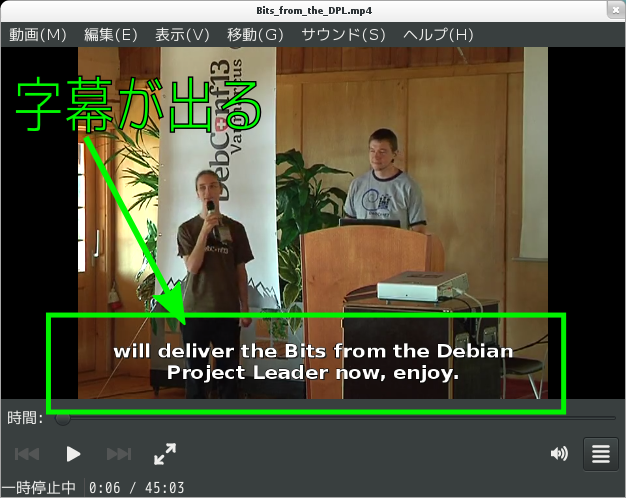
\includegraphics[scale=0.25]{image201310/totem-subtitle.png}
\end{center}

\end{frame}

\begin{frame}{Debian Conference 2013トピック紹介}
\begin{center}
\LARGE
とりあえず、見どころをいくつか
\end{center}
\end{frame}

\begin{frame}{Bit from the Debian Project Leader 1/2}

 まずは、''Bit from the Debian Project Leader''から、
(プレゼン資料:\url{http://www.lucas-nussbaum.net/blog/wp-content/uploads/2013/08/bits.pdf})
\begin{enumerate}
\item Debianの紹介と、現在のDebianのコミュニティの様子について説明(割と宣伝な感じです)
\item 現在のDebianの課題と提案
\begin{itemize}
  \item CloudのIaaS/PaaS/SaaS環境の元でどうやって自由を獲得するのか?
  \item テスト版(testing)を利用してローリングリリースとしたらどうか?(もちろん、安定版(stable)はちゃんと残す)
  \item いろいろマンパワーが足らないので、とにかく新しい開発者/貢献してくれる人を捕まえよう
 \item Debianの運営について、DPLの負荷減らしも含めて、もっとうまいこと改善したい。
\end{itemize}
\end{enumerate}

\end{frame}

\begin{frame}{Bit from the Debian Project Leader 2/2}

テスト版(testing)使ったローリングリリースの件は、皆さん関心が大変高いようで、

\begin{center}
\LARGE
質疑応答がすべてローリングリリースの件になってました...
\end{center}

\end{frame}

\begin{frame}{Lightning talk}

 Debconf13のLightning talkがおもしろかったのでいくつか...

\begin{itemize}
\item Coqelicot \\
\url{https://coquelicot.potager.org}\\
※Coqelicotはフランス語でひなげしの花の意味\\
いわゆるWebベースのファイル共有サービスのプログラムを作ったとのこと。
特徴として、ファイルは全部暗号化されてストア(しかも暗号化キーはストアされない)、
時間がたてば自動で消去、消去の時にはzeroで埋めるなどの
特徴がある。ライセンスはAGPL。
\item notmuch \\
\url{http://notmuchmail.org/}
大量のメールを高速に扱うためのソフトウェアの紹介。
vim/emacsのフロントエンドなどもある。タグづけにも対応。
\end{itemize}

\end{frame}

\begin{frame}{Lightning talk}

\begin{itemize}
\item  messaging bus system for debian infrastracture\\
\url{http://www.fedmsg.com/en/latest/}\\
Fedora PJのインフラを支えるために作られたメッセージバスシステムの紹介。
Debianにもいかが?という内容。
debianを支えるいろいろなインフラ上の仕組み(ftpキューとか、bugreportとか)
で発生する様々なイベントをこのバスシステムに流し込むと、いろいろなメディア
に柔軟に接続することができる。\\
(例:ftpキューでリジェクトされたら、WEBにも出るとかのシステムが作りやすく
 なる)\\
\url{http://www.fedmsg.com/en/latest/topology/}
を観るとわかりやすい。また、\\
繋げることができるようになったシステムの一覧↓\\
\url{http://www.fedmsg.com/en/latest/status/}
発表長すぎて司会(ドラ娘)に止められたのが残念。
\end{itemize}
\end{frame}

\begin{frame}{Lightning talk}
\begin{itemize}
\item dedup.debian.netの紹介\\
\url{http://dedup.debian.net/}\\
バイナリパッケージ内部のファイルのmd5sumとかsha1とかのハッシュ
をとり、他のバイナリパッケージに重複したものがあるかどうかを
調べるサイトの紹介。例として、freefem++,calibreの
パッケージについて、どの程度他パッケージにも含まれている
ファイルがあるかをデモ。gzipされたファイルも元ファイルの
md5sumなどを取って比較できる。\\
例:\url{http://dedup.debian.net/binary/freefem++}\\
    \url{http://debdup.debian.net/compare/calibre/python-odf}\\
   (calibreとpython-odfは見てのとおり重複しまくり)\\
\end{itemize}
\end{frame}

\begin{frame}{Lightning talk}
\begin{itemize}
\item Skarphed - Webmanagement system\\
\url{http://www.skarphed.org/}\\
Webサイトを非常に簡単に構築できるシステムを開発したとのことで、そのデモの紹介。  
登録したサーバーに、非常に簡単にWebサイトを構築できる。AGPLで提供とのこと。
\item organaize of your life with org mode.\\
\url{http://orgmode.org/ja/}\\
emacsで動く、独特なテキスト文章作成環境のデモ。今回プレゼンすら、org modeでやった。
見ればわかりますが、TODO作成など、とても便利そうな印象を受けます。
\end{itemize}

\end{frame}

\begin{frame}{Lightning talk}
\begin{itemize}
\item openhatch\\
\url{https://openhatch.org}\\
fossの貢献者らのためのfossプロジェクトマッチングサービスの紹介。
Web上で、fossに貢献するために必要な基本的なスキルトレーニングを
つむ、難易度に応じたfossプロジェクトを紹介する、イベントを紹介する
などのサービスが受けられる。
\end{itemize}
\end{frame}

\begin{frame}
\begin{center}
\LARGE{イベントのご紹介}
\end{center}
\end{frame}

\begin{frame}{東京エリア/関西エリア/福岡 Debian勉強会}

\begin{itemize}
\item 東京エリアDebian勉強会\\
\url{http://tokyodebian.alioth.debian.org}
\item 関西エリアDebian勉強会\\
\url{http://wiki.debian.org/KansaiDebianMeeting}
\item 福岡Debian勉強会\\
\url{http://fukuoka-debian.github.io/web/}
\end{itemize}

\begin{center}
\Large
場所、お時間が合えば、ぜひお越し下さい。
\end{center}

\end{frame}

\begin{frame}{その他イベント}

\begin{center}
\Large
 その他、いろいろなDebian関係のイベントはこちら\\
\url{http://www.debian.or.jp/}\\
Twitter: @debianjp 

\end{center}

\end{frame}

\begin{frame}{本日の展示}
\begin{center}
\Large
本日東京エリアDebian勉強会のブースだしてます。
\end{center}
展示物:
\begin{enumerate}
\item Wheezy PCの展示
\item あんどきゅめんてっどでびあんの展示/頒布
\item Debianステッカーの配布
\item Debian インストール CDの配布
\item 東京エリア/関西Debian勉強会の紹介
\end{enumerate}
\begin{center}
\Large
是非、お立ち寄りくださいませー
\end{center}

\end{frame}

\begin{frame}{質疑応答}
\begin{center}
\Large なにか質問はありますか?
\end{center}
\end{frame}



\end{document}

;;; Local Variables: ***
;;; outline-regexp: "\\([ 	]*\\\\\\(documentstyle\\|documentclass\\|emtext\\|section\\|begin{frame}\\)\\*?[ 	]*[[{]\\|[]+\\)" ***
;;; End: ***
